\chapter{Hauptteil}

\section{Architektur der Applikation}

\begin{figure}
	\centering
	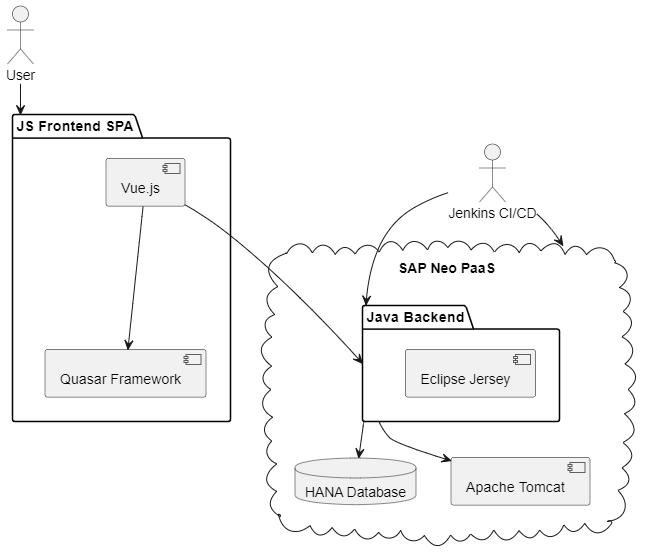
\includegraphics[width=.72\textwidth]{Bilder/architecture.png} 
	\caption{Die Abbildung zeigt die Architektur der Digital Heroes Lernplattform.}
	\label{fig:architecture}
\end{figure} 

Die Architektur der Web-App Digital Heroes mit den verschiedenen verwendeten Technologien
lässt sich in Frontend, Backend und DevOps unterteilen und 
ist in \autoref{fig:architecture} abgebildet. 
Es existieren zwei Instanzen der Architektur: ein Entwicklungs- und ein Produktivsystem. 

\subsubsection*{Frontend:}

Die Frontend-Anwendung der Digital Heroes Web-App ist als Single Page Application (SPA) konzipiert, 
die Vue.js und das Quasar Framework verwendet. 
Vue.js ist ein modernes JavaScript-Framework zum Erstellen von benutzerfreundlichen und reaktiven Webanwendungen.
Quasar ist ein weiteres Framework, das auf Vue.js aufbaut und zusätzliche Funktionen und Komponenten bereitstellt, 
um die Entwicklung von plattformübergreifenden Anwendungen zu erleichtern.
Vue.js nutzt die REST-API des Backends.

\subsubsection*{Backend:}

Das Backend der Web-App besteht aus einer Java-Anwendung, die Eclipse Jersey und Apache Tomcat verwendet. 
Eclipse Jersey ist eine Implementierung der JAX-RS-Spezifikation 
und ermöglicht die einfache Entwicklung von RESTful Web Services für Servlet Container. 
Apache Tomcat ist ein Servlet-Container, der als Webserver zum Bereitstellen von Java-Anwendungen dient
und das Java-Backend hostet.
Als Datenbank kommt die HANA-Datenbank zum Einsatz, die eine high-performance, in-memory relationale Datenbank ist 
und von SAP entwickelt wird. 
Das Java-Backend nutzt das Eclipse-Framework und die HANA-Datenbank um eine REST-API für das 
Vue.js-Frontend bereitzustellen. 

\subsubsection*{DevOps:}

Im Bereich der DevOps-Infrastruktur kommt Jenkins zum Einsatz, 
eine Open-Source-Automatisierungssoftware, 
die zur Implementierung von Continuous Integration und Continuous Deployment (CI/CD) verwendet wird. 
Jenkins ermöglicht die Automatisierung von Build- und Testprozessen sowie die Bereitstellung 
der Anwendung in einer kontrollierten und konsistenten Weise. 
Die Web-App wird auf der SAP Neo Platform-as-a-Service (PaaS) Cloud-Plattform gehostet, 
die eine skalierbare und einfach zu verwaltende Umgebung für die Bereitstellung 
und den Betrieb der Anwendung bietet.
Wird auf den Main-Branch des verwendeten Github-Respositories gepusht, bzw. eine Pull-Request gemerged,
startet Jenkins den CI/CD-Prozess und testet und deployed das neue Backend/Frontend auf der Entwicklungsinstanz. 
Änderungen im Frontend werden zudem direkt auf dem Produktivsystem deployed. 
Für Änderungen des Backends im Produktivsystem kann in SAP Neo ein neuer Release erzeugt werden, 
bei dem das Java-Backend der Entwicklungsinstanz auf das Produktivsystem kopiert wird. 